\documentclass[12pt]{article}

\usepackage{tikz} % картинки в tikz
\usepackage{microtype} % свешивание пунктуации

\usepackage{array} % для столбцов фиксированной ширины

\usepackage{indentfirst} % отступ в первом параграфе
\usepackage{verbatim} % для комментов

\usepackage{sectsty} % для центрирования названий частей
\allsectionsfont{\centering}

\usepackage{amsmath} % куча стандартных математических плюшек

\usepackage{comment}

\usepackage[top=2cm, left=1.2cm, right=1.2cm, bottom=2cm]{geometry} % размер текста на странице

\usepackage{lastpage} % чтобы узнать номер последней страницы

\usepackage{enumitem} % дополнительные плюшки для списков
%  например \begin{enumerate}[resume] позволяет продолжить нумерацию в новом списке
\usepackage{caption}


\usepackage{fancyhdr} % весёлые колонтитулы
\pagestyle{fancy}
\lhead{Теория вероятностей}
\chead{}
\rhead{2017-12-09, Финик или Груша}
\lfoot{}
\cfoot{}
\rfoot{\thepage/\pageref{LastPage}}
\renewcommand{\headrulewidth}{0.4pt}
\renewcommand{\footrulewidth}{0.4pt}



\usepackage{todonotes} % для вставки в документ заметок о том, что осталось сделать
% \todo{Здесь надо коэффициенты исправить}
% \missingfigure{Здесь будет Последний день Помпеи}
% \listoftodos --- печатает все поставленные \todo'шки


% более красивые таблицы
\usepackage{booktabs}
% заповеди из докупентации:
% 1. Не используйте вертикальные линни
% 2. Не используйте двойные линии
% 3. Единицы измерения - в шапку таблицы
% 4. Не сокращайте .1 вместо 0.1
% 5. Повторяющееся значение повторяйте, а не говорите "то же"



\usepackage{fontspec}
\usepackage{polyglossia}

\setmainlanguage{russian}
\setotherlanguages{english}

% download "Linux Libertine" fonts:
% http://www.linuxlibertine.org/index.php?id=91&L=1
\setmainfont{Linux Libertine O} % or Helvetica, Arial, Cambria
% why do we need \newfontfamily:
% http://tex.stackexchange.com/questions/91507/
\newfontfamily{\cyrillicfonttt}{Linux Libertine O}

\AddEnumerateCounter{\asbuk}{\russian@alph}{щ} % для списков с русскими буквами
\setlist[enumerate, 2]{label=\asbuk*),ref=\asbuk*}

%% эконометрические сокращения
\DeclareMathOperator{\Cov}{Cov}
\DeclareMathOperator{\Corr}{Corr}
\DeclareMathOperator{\Var}{Var}
\DeclareMathOperator{\E}{E}
\def \P{P}
\def \hb{\hat{\beta}}
\def \hs{\hat{\sigma}}
\def \htheta{\hat{\theta}}
\def \s{\sigma}
\def \hy{\hat{y}}
\def \hY{\hat{Y}}
\def \v1{\vec{1}}
\def \e{\varepsilon}
\def \he{\hat{\e}}
\def \z{z}
\def \hVar{\widehat{\Var}}
\def \hCorr{\widehat{\Corr}}
\def \hCov{\widehat{\Cov}}
\def \cN{\mathcal{N}}

\newenvironment{problem}{}{}

% тут перещёлкиваем комментарий, чтобы убрать или показать решения:
\newenvironment{sol}{}{} % with solutions
% \excludecomment{sol} % without solutions


\begin{document}
% карты 
% https://docs.google.com/spreadsheets/d/1woBHzicny2SJ6hoZcbJZpcFHD6fMQZon4N9SSk0Z_wk/edit#gid=289446287

\section{Тур 1}

\subsection{Тур 1 — Основная часть — Дискретные распределения}

\begin{enumerate}
% тур 1 - основная часть - дискретные распределения
\begin{problem}
\item[A1.] После смерти Мориарти на крыше Шерлоку нужно срочно вспомнить заранее обговорённое для такого исхода кодовое слово. Однако Шерлок так расстроился от смерти Джима, что совсем забыл то самое слово! К счастью, у Шерлока есть чертоги разума, в которых есть картинка кодового слова, но, почему-то, на греческом: \textbf{Λάζαρος} . К сожалению, Шерлок не изучал теорию вероятностей на экономе Вышки и плохо помнит греческий алфавит, вероятность вспомнить аналог буквы на латинице равна $0.8$, а раскладку на своём Blackberry он поменять не может.

\begin{enumerate}
\item Напишите кодовое слово русскими буквами.
\item Найдите вероятность того, что Шерлок отправит неправильное смс и не спасётся.
\end{enumerate}
\begin{sol}
\textbf{Внимание! Это задача-сюрприз!} Забираем в студию, если задача решена неверно.

Лазарос (Лазарь), $1-0.8^7$
\end{sol}
\end{problem}

% тур 1 - основная часть - дискретные распределения
\begin{problem}
\item[A2.] Мориарти объявил начало «Большой игры» — в течение $n$ дней каждый день его криминальными бандами будет свершаться преступление с вероятностью $p$ (независимо друг от друга). Бравые детективы Шерлок и Джон раскрывают каждое преступление с вероятностью $r$ (тоже независимо от предыдущих дней).
\begin{enumerate}
\item Найдите функцию распределения количества совершенных преступлений.
\item Найдите функцию распределения количества раскрытых преступлений. 
\end{enumerate}

\begin{sol}
$\P(X = k) = C^{\ k}_{\ n} (p)^k(1-p)^{n-k}$, \ $\P(Y = k) = C^{\ k}_{\ n}  (pr)^k(1-rp)^{n-k}$
\end{sol}
\end{problem}

% тур 1 - основная часть - дискретные распределения
\begin{problem}
\item[A3.]
Шерлок и Джон соперничают всю неделю и хотят выяснить, кто быстрее догадывается о личности настоящего убийцы. Пусть выигрывает тот, кто первым отгадал убийцу 4 раза подряд. $p$ — вероятность, что Джон оказался догадливее Шерлока и в конкретном деле быстрее вычислил виновного. Найдите вероятность того, что Джон выиграл во всей игре.

\begin{sol}
$\P(\text{Джон выигрывает}) = C^4_7p^4q^3 +C^5_7p^5q^2+C^6_7p^6q+p^7$ 
\end{sol}
\end{problem}

% тур 1 - основная часть - дискретные распределения
\begin{problem}
\item[A4.]
Ирэн и Шерлок очень любят писать друг другу смски, но стесняются показать свою привязанность. Шерлок подбрасывает монетку $n$ раз, а Ирэн — $n + 1$ раз. Оба придерживаются следующей стратегии: когда выпадает орёл, он/она отправляют смску, когда решка — ничего не отправляют. Найдите вероятность того, что Ирэн отправила больше смсок, чем Шерлок.

\begin{sol}
$1/2$
\end{sol}
\end{problem}

% тур 1 - основная часть - дискретные распределения
\begin{problem}
\item[A5.]
Шерлок пытается найти нужную информацию в чертогах разума. Пусть он находит её с вероятностью $p$ за одну попытку и не находит с вероятностью $q=1 -p$. $X$ — число попыток, которое понадобилось Шерлоку. Найдите $\E\left(\frac{1}{X+1} \right)$.

\begin{sol}
$- \frac{p}{q} \ln p$
\end{sol}
\end{problem}




\end{enumerate}

\newpage
\subsection{Тур 1 — Основная часть — Комбинаторика}

\begin{enumerate}

% тур 1 - основная часть - комбинаторика
\begin{problem}
\item[B1.] ОБН прослушивает телефон Джесси Пинкмана, поэтому он решил отправить закодированное послание мистеру Уайту, чтобы сохранить в секрете место следующей встречи. Для дополнительной секретности он составляет текст на русском языке, а потом кодирует каждую букву последовательностью из нулей и единиц длины $n$. Он хочет отправить послание как можно скорее и исключить неоднозначность раскодирования, поэтому выбирает наименьшее подходящее $n$. Чему оно равно?

\begin{sol}
$6$
\end{sol}
\end{problem}

% тур 1 - основная часть - комбинаторика
\begin{problem}
\item[B2.] Хэнк и Уолтер решили сыграть в следующую игру: каждый по очереди называет такую расстановку пяти ладей на шахматной доске, что ни они не бьют друг друга. Начинает Хэнк. Сколько ходов возможно сделать в этой игре, если играть до самого конца, а повторять уже названные расстановки нельзя.

\begin{sol}
$64 \cdot 49 \cdot 36 \cdot25 \cdot 16$ или $45\,158\,400$
\end{sol}
\end{problem}

% тур 1 - основная часть - комбинаторика
\begin{problem}
\item[B3.] Вернемся к сюжету из первой задачи. Все понимают, что Джесси может иногда совершить ошибку, пока кодирует свое послание. Поэтому теперь мистер Уайт и Джесси хотят так кодировать символ, чтобы даже при совершении Джесси ошибки в одном знаке можно было правильно раскодировать символ. Какого $n$ им будет достаточно сейчас? 

\begin{sol}
\textbf{Внимание! Это задача-сюрприз!} Предлагаем на выбор: частичный балл за какую-нибудь задачу / освобождение участника из студии

$9$
\end{sol}
\end{problem}

% тур 1 - основная часть - комбинаторика — Клад!
\begin{problem}
\item[B4.] Уолт поспорил с сыном, сможет ли он расставить числа от 1 до 2016 по кругу так, чтобы все суммы соседних чисел были разными. Выиграет ли он в споре и почему?

\begin{sol}
\textbf{Ответ:} да, выиграет

\textbf{Решение:} Рассмотрим расстановку $1, 2, 3,\hdots, 2014, 2016, 2015$. Выпишем суммы соседних чисел: $1+2 = 3, 2+3 = 5, 3+4 = 7,\hdots, 2013+2014 = 4027, 2014+
2016 = 4030, 2016 + 2015 = 4029, 2015 + 1 = 2016$. В этом списке по одному
разу появятся нечетные числа $3, 5,\hdots, 4027, 4029$ и четные $4030, 2016$.
\end{sol}
\end{problem}

% тур 1 - основная часть - комбинаторика
\begin{problem}
\item[B5.] Уолт собирается оставить свой уличный бизнес одному из 3 бывших учеников. У первого ученика есть два наследника, у второго — три, а у третьего — пять. Всем известно, что Уолт скоро объявит, кто именно сменит его на уличном престоле. На какое наименьшее количество районов можно разделить город так, чтобы при любом выборе Уолта, новый властитель мог бы раздать все округа своим наследникам, и каждому из них досталась бы территория одинаковой площади?

\begin{sol}
8
\end{sol}
\end{problem}
\end{enumerate}



\newpage
\subsection{Тур 1 — Основная часть — Метод первого шага}

\begin{enumerate}
% тур 1 - основная часть - метод первого шага
\begin{problem}
\item[C1.] Джоуи решил посмотреть телевизор после очередных неудачных проб на роль в сериале. Сейчас по телевизору идут новости. Джоуи переключает каналы в поисках футбольного матча, при этом известно, что на каждом канале показывают футбол с вероятностью $p=0.7$ и новости с вероятностью $1-p=0.3$. Пусть $X -$ это количество каналов, которые посмотрел Джоуи, прежде чем нашёл футбольный матч. Найдите $\E(X), \E(X^2), \Var(X)$ методом первого шага.

\begin{sol}
$\frac{10}{7},\frac{130}{49},\frac{30}{49}$
\end{sol}
\end{problem}

% тур 1 - основная часть - метод первого шага
\begin{problem}
\item[C2.] Фиби и Чендлер решили посмотреть телевизор после ссоры с Джоуи. Они включают телевизор и видят, что сейчас как раз идет фильм с ним. Фиби переключает каналы в поисках мультиков, при этом при переключении каналов действует следующее правило: при нечётном переключении канала Фиби попадёт на мультики с вероятностью $p=0.5$ и на фильм с Джоуи с вероятностью $1-p=0.5$, а при чётном — с вероятностями $p=0.75$ и $1-p=0.25$ соответственно. Пусть $X$ — это количество каналов, которые посмотрела Фиби, прежде чем нашла мультики. Найдите $\E(X), \E(X^2), \Var(X)$ методом первого шага.

\begin{sol}
$\frac{12}{7},\frac{164}{49},\frac{20}{49}$
\end{sol}
\end{problem}

% тур 1 - основная часть - метод первого шага — Клад!
\begin{problem}
\item[C3.] Росс подкидывает правильную монетку. Если монетка выпадает орлом, Росс генерирует случайную величину $X\sim \cN(1,\sigma^2)$, если монетка выпадает решкой, Росс> подкидывает монетку заново. Если монетка на этот раз выпадает орлом, Чендлер генерирует случайную величину $X\sim \cN(\frac{1}{2},\frac{1}{4}\sigma^2)$, иначе подкидывает монетку заново. В общем случае если монетка выпадает орлом на $n$-тое подкидывание, Чендлер  генерирует случайную величину $X\sim \cN \left(\frac{1}{2^{n-1}},\frac{1}{4^{n-1}}\sigma^2 \right)$. Найдите $\E(X), \E(X^2)$ методом первого шага.

\begin{sol}
\textbf{Ответ:} $\frac{2}{3},\frac{4(\sigma^2+1)}{7}$

\textbf{Решение:} Заметим, что на $n$-том шаге случайную величину $X$ можно представить как: $X = \frac{1}{2^{n-1}}+\frac{1}{2^{n-1}}\sigma^\cdot\varepsilon,\;\; \varepsilon\sim \cN(0,1)$, поэтому
\[
\E(X)= 0.5\cdot \E(1+\sigma\cdot \cN(0,1)) + 0.5\cdot \E\left(\frac{X}{2}\right)   \rightarrow \E(X)=\frac{2}{3}
\]
\[
\E(X^2)= 0.5\cdot \E((1+\sigma\cdot \cN(0,1))^2) + 0.5\cdot \E\left(\frac{X^2}{4}\right)
\rightarrow \E(X^2)=\frac{4(\sigma^2+1)}{7}
\]
\[
(Z\sim \cN(\mu,\sigma^2)\rightarrow \E(Z^2)=\mu^2 + \sigma^2)
\]
\end{sol}
\end{problem}


% тур 1 - основная часть - метод первого шага
\begin{problem}
\item[C5.] На свадьбе у Рэйчел женская часть гостей выстроились в линию чтобы ловить букет. В линии в случайном порядке стоят $n$ девушек, все разного роста. Моника  опаздывает и не успевает встать в ряд, поэтому ей удаётся посмотреть на всю линию только сбоку. Сколько в среднем жаждущих выйти замуж девушек увидит Моника? 

\begin{sol}
$1+\frac{1}{2}+\dots+\frac{1}{n}$
\end{sol}
\end{problem}
\end{enumerate}

\newpage
\subsection{Тур 1 — Основная часть — Неравенства Чебышёва и Маркова}


\begin{enumerate}
% тур 1 – основная часть – неравенства
\begin{problem}
\item[D1.] Вы Раджеш Кутрапали и у вас проблемы в общении с девушками. Если вы не выпьете алкоголь, то вы не можете разговаривать с женщинами. Каждые пол минуты вы равновероятно делаете глоток пива или нет. Если вы сделаете более 25 глотков, то вы дойдёте до нужной кондиции. Оцените сверху вероятность того, что через 20 минут Раджеш сможет говорить с прекрасной половиной человечества. 

\begin{sol}
$\P(\text{Радж готов}=True) \leq 0.8$
\end{sol}
\end{problem}

% тур 1 – основная часть – неравенства
\begin{problem}
\item[D2.] Вы команда кафедры теоретической физики по страйкболу, вы должны защитить честь кафедры на чемпионате по страйкболу ведь в нём участвуют географы, биологи и, что самой ужасное, гуманитарии. В вашей команде четверо человек. В команде гуманитариев 6 человек. Говорят, что на одного павшего в страйкболе приходится в среднем 100 шариков. Сколько нужно вам взять шариков в среднем на человека, чтобы оценка сверху убийства не менее 6 человек в неравенстве Маркова была равна 1? Для простоты считайтйе, что вы все переживёте эту бойню.

\begin{sol}
\textbf{Внимание! Это задача-сюрприз!} Предлагаем на выбор: -5 минут от времени клада / -5 очков команде-сопернику

Не менее 150 на человека.
\end{sol}
\end{problem}

% тур 1 – основная часть – неравенства
\begin{problem}
\item[D3.] Вы Говард Воловиц инженер с всего лишь степенью магистра. Вы конструируете робота, у которого имеется 100 узлов, которые могут сломаться за время автономной работы с вероятностью в 10\%. Оцените сверху вероятность того, что число поломанных узлов будет отличаться от ожидаемого более чем на 5 узлов. 

\begin{sol}
$\P(\vert \text{Поломок} - \E(\text{Поломок}) \vert  >5) \leq 9/25$
\end{sol}
\end{problem}

% тур 1 – основная часть – неравенства
\begin{problem}
\item[D4.] Вы Пенни, весьма милая девушка без высшего образования. Но вы переобщались с Шелдоном Купером. Из-за этого в вашей голове возникла задачка. Вы знаете, что каждые 20 минут у вас на работе заказывают два сырника с вероятностью $1/4$ и с такой же не заказывают, с оставшейся вероятностью у вас берут один сырник. Ваша смена длится 6 часов. Вы хотите оценить сверху вероятность того, что у вас закажут более 24 или менее 12 сырников. 

\begin{sol}
$\P(\vert \text{Сырников за смену} - \E(\text{Сырников за смену}) \vert  >6) \leq 1/4$
\end{sol}
\end{problem}

% тур 1 – основная часть – неравенства
\begin{problem}
\item[D5.] Вы Бернадетт Мэри Энн Ростенковски-Воловиц, микробиолог и вы скрестили Эболу с гриппом, но этого не было. Вы знаете что за условный период времени число бактерий возрастает либо в 2.71 раз либо в 7.39 раз равновероятно. Оцените снизу вероятность того что число бактерий за 20 условных периодов возрастет от $e^{25}$ до $e^{35}$ раз.

\begin{sol}
$\P(e^{25} \leq \text{Рост} \leq e^{35}) \geq 0.8 $ 
\end{sol}
\end{problem}


\end{enumerate}

\newpage
\subsection{Тур 1 — Основная часть — Условные вероятности}

\begin{enumerate}
% тур 1 - основная часть - условные вероятности
\begin{problem}
\item[E1.] Мы знаем, что кроме Элевен в Национальной лаборатории Хоукинса были еще дети. Предположим, в самом начале экспериментов было двое детей, один из которых был мальчиком. Если предположить, что Доктор Бреннан мог похитить равновероятно мальчика или девочку, то какова вероятность, что второй ребенок тоже был мальчиком?

\begin{sol}
$\frac{1}{3}$
\end{sol}
\end{problem}

% тур 1 - основная часть - условные вероятности
\begin{problem}
\item[E2] Из 100 опрошенных жителей Хоукинса, 30 работают в Национальной лаборатории Хоукинса, из которых 10 знают о том, что был открыт проход на «ту сторону». Какова вероятность, что если опрошенный житель работает в лаборатории, то он знает о проходе?

\begin{sol}
$\frac{1}{3}$
\end{sol}
\end{problem}

% тур 1 - основная часть - условные вероятности
\begin{problem}
\item[E3.] Встретившись лицом к лицу с Демогоргном, Дастин Лукас и Майк используют против него единственное оружие, которое у них есть — рогатки. Все трое напуганы и стреляют независимо. Дастин попадает с вероятностью $\frac{1}{4}$, Майк — с вероятностью $\frac{1}{6}$, А Лукас — с вероятностью $\frac{1}{3}$.

\begin{enumerate}
\item Какова вероятность, что только один из них попадет в монстра?
\item Каковая вероятность, что попадет Лукас, если попал только один из ребят?
\end{enumerate}

\begin{sol}
a) $\frac{31}{72}$; б) $\frac{15}{31} $
\end{sol}
\end{problem}

% тур 1 - основная часть - условные вероятности
\begin{problem}
\item[E4.]  Дастин, Лукас, Майк и Уилл играют в Dungeons and Dragons в подвале у Майка. Из 25 игральных карт, дающих специальные способности, 5 карты дают рунные заклинания, которые помогут пройти сквозь лес с демодогами. Ребята вытягивают карты по очереди. У кого больше вероятность вытащить счастливый билет: у Уилла (он тянул первый), или Лукаса (тянул вторым)?

\begin{sol}
\textbf{Внимание! Это задача-сюрприз!} Предлагаем на выбор: стикеры / возможность открыть клетку, к которой нет пути (десант!)

$\P(L|W)=\frac{4}{24}, \P(L|W^{c})=\frac{5}{24}, \P(W)=\frac{1}{5}, \P(W^{c})=\frac{4}{5} \\
\P(L)=\frac{4}{24}\frac{1}{5}+\frac{5}{24}\frac{4}{5} = \frac{1}{5}= \P(W)$. Вероятность одинаковая.
\end{sol}
\end{problem}

% тур 1 - основная часть - условные вероятности
\begin{problem}
\item[E5.] Дастин и Макс играют в игровые автоматы. Дневной матч состоит из серии игр, причем $p$ — вероятность Дастина выиграть каждую игру (независимо). Первый, кто выигрывает на две игры больше противника, становится победителем дня. Какова вероятность того, что Дастин выиграет дневной матч (в терминах $p$)?

\begin{sol}
$\P(D) = \frac{p^2}{1-2pq}=\frac{p^2}{p^2+q^2}$
\end{sol}
\end{problem}

\end{enumerate}




\newpage
\subsection{Тур 1 — студия — Ковариации и корреляции}

\begin{enumerate}

% тур 1 - студия - ковариации и корреляции
\begin{problem}
\item[A1.] Создатель правой палочки и создатель левой палочки Twix бросают одновременно правильный десятигранный шоколадный кубик. Пусть $X$ и $Y$ значения, которые выпали создателю правой и левой палочки соответственно.

Найдите ковариацию между $X+Y$ и $X-Y$.

\begin{sol}
$\Cov(X+Y,X-Y) = 0 $
\end{sol}
\end{problem}

% тур 1 - студия - ковариации и корреляции
\begin{problem}
\item[A2.] Вы пошли на интервью, для того, чтобы сниматься в рекламе Альпен Гольда. Вы очень понравились жюри, но они хотят проверить ваше знание статистики. Вам дают такую задачу.

Пусть $\E(X) = 3, \E(\lambda) = -2, \Var(X) = 1,\E(\lambda^2) = 8, \E(X\lambda) = -1$
Найдите $\Cov(X,\lambda), \Corr(X,\lambda)$

\begin{sol}
$\Cov(X,\lambda) = 5, \Corr(X,\lambda)= 2.5$.
\end{sol}
\end{problem}

% тур 1 - студия - ковариации и корреляции
\begin{problem}
\item[A3.] Верны ли следующие утверждения?

\begin{enumerate}
\item Некоррелированные нормально распределенные случайные величины независимы.
\item Случайные величины $X$ и $Y$ зависимы, $Y$ и $Z$ зависимы. Верно ли, что случайные величины $X$ и $Z$ зависимы?
\end{enumerate}

\begin{sol}
а) Нет, б) Нет
\end{sol}
\end{problem}

% тур 1 - студия - ковариации и корреляции
\begin{problem}
\item[A4.] Вы пытаетесь оценивать зависимость между продажами Сникерса и печенья. Вам известно количество продаж в $100$ магазинах (нарисованы на графике). По оси $OX$ количество проданных Сникерсов, по оси $OY$ продажи печенья. 

Существует ли зависимость между продажами Сникерса и печенья? Какой знак у корреляции? 

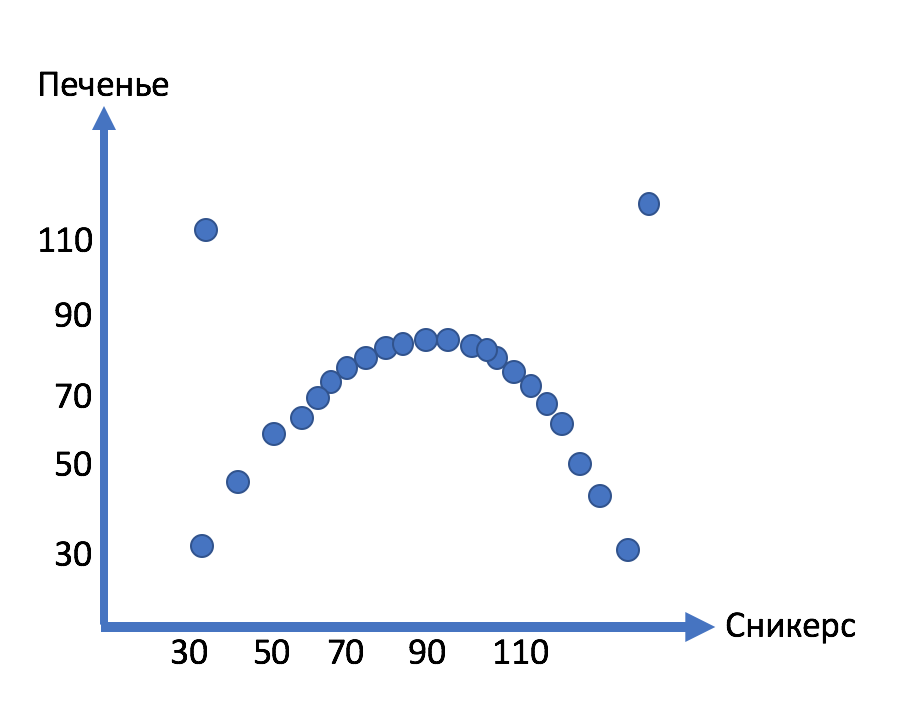
\includegraphics[scale=0.5]{No_correlation}

\begin{sol}
$X$ и $Y$ зависимы, но корреляция равна $0$.
\end{sol}
\end{problem}
\end{enumerate}


\newpage
\subsection{Тур 1 — студия — Нормальное распределение}

\begin{enumerate}
\begin{problem}
\item[B1.] Микрофинансовая организация <<Рабочие деньги>> обычно предлагает займы под \(144\%\) годовых. По случаю своего дня рождения она решила устроить акцию: для одного счастливчика ставка будет равна не \(144\%\) годовых, а реализации случайной величины \(X\sim \mathcal{N}(144; 1296)\). Найдите вероятность того, что ставка для счастливчика превысит \(180\%\) годовых.

\begin{sol}
$\approx 0.1586553$
\end{sol}
\end{problem}

\begin{problem}
\item[B2.] Директор «Рабочих денег» Иннокентий, пытается оценить, как распределены доходы его заёмщиков. Он считает, что распределение нормальное, но не уверен, какие у него параметры. Иннокентий нарисовал две функции распределения: $\cN(10000, 5000)$ и $\cN(12500, 15)$. Воспроизведите схематично рисунок Иннокентия.

\begin{sol}
$\cN(10000, 5000)$ — колокол, симметричный относительно прямой $x=10000$, с маленьким горбом; $\cN(12500, 15)$ — колокол, симметричный относительно прямой $x=12500$ с очень острым и узким горбом.
\end{sol}
\end{problem}

\begin{problem}
\item[B3.] На номер 8 800-555-35-35 поступил звонок от Валерия. Как хорошо, что Иннокентий заранее определился с распределением доходов своих клиентов! Доход каждого – случайная величина, распределённая нормально с математическим ожиданием $15000$. Проведя беглый опрос, Иннокентий прикинул вероятность того, что истинный доход Валерия лежит в интервале $(12000, 13000)$. По его оценке, она равна $0.3$. А какова вероятность того, что истинный доход Валерия лежит в интервале $(17000, 18000)$?

\begin{sol}
$0.3$
\end{sol}
\end{problem}

\begin{problem}
\item[B4.] Иннокентий снова делает квартальный отчёт. В этот раз он уверен, что распределение доходов заёмщиков – нормальное с матожиданием $20000$ и стандартным отклонением $1000$. Но он совсем забыл функцию плотности нормального распределения, поэтому написал смс жене: «Котя, напомни функцию плотности нормального распределения, плз». Помогите Иннокентию, плз.

\begin{sol}
$f(x) = \frac{1}{\sqrt{2 \pi 1000^2}}e^{-\frac{1}{2}\cdot \frac{(x-20000)^2}{1000^2}}$
\end{sol}
\end{problem}

\end{enumerate}


\newpage
\subsection{Тур 1 — студия — Непрерывные распределения}

\begin{enumerate}
% тур 1 - студия - непрерывные распределения
\begin{problem}
\item[C1.] Количество сиреневых конфет Skittles в каждой пачке – равномерная на отрезке $[0; \pi]$ случайная величина. Найдите $\P(\min\{X_1, \ldots, X_{1000}\} > e)$.

\begin{sol}
$\left(\frac{\pi - e}{\pi}\right)^{1000}$
\end{sol}
\end{problem}

% тур 1 - студия - непрерывные распределения
\begin{problem}
\item[C2.] Растаман в рекламе Skittles доит жирафа. Доля конфет красного цвета в надое – случайная величина и имеет следующую функцию распределения:

\[
F(x)  = \begin{cases}
C_1, & x < 0 \\
0.5 x^2 + 0.5x + C_3, & x\in [0,1] \\
C_2, & x > 1
\end{cases}
\]
Найдите $C_3$.

\begin{sol}
$0$
\end{sol}
\end{problem}

% тур 1 - студия - непрерывные распределения
\begin{problem}
\item[C3.] Количество сахара в граммах в конфете Skittles — случайная величина с функцией распределения $F(x) = \frac{1}{2} + \frac{\arctan(x)}{\pi}$. Найдите $\P(0<X<1)$.

\begin{sol}
$\frac{1}{4}$
\end{sol}
\end{problem}

% тур 1 - студия - непрерывные распределения
\begin{problem}
\item[C4.] Чтобы рассмотреть всю радугу, жирафу, стоящему прямо перед ней, нужно наклонять голову вправо или влево. Угол наклона головы – случайная величина $X$ с функцией плотности:

\[
f(x) = \begin{cases}
\frac{2}{\pi} \cos^2 x & x \in \left[-\frac{\pi}{2}, \frac{\pi}{2}\right] \\
0 & \text{иначе}
\end{cases}
\]

Жираф наклоняет трижды. Найдите вероятность того, что ровно два раза угол наклона будет лежать в интервале $\left(0, \frac{\pi}{4}\right)$.

\begin{sol}
$C_3^2 \left(\frac{2+\pi}{4\pi}\right)^2 \frac{3\pi-2}{4\pi}$
\end{sol}
\end{problem}
\end{enumerate}


\newpage
\subsection{Тур 1 — студия — Оптимальные стратегии}

\begin{enumerate}
% тур 1 - студия - оптимальные стратегии
\begin{problem}
\item[D1.] Леонид Якубович подбрасывает неправильную монетку и каждый раз пытается угадать, как она выпадет. В качестве прогноза на следующий бросок он использует результат предыдущего броска. Монетка выпадает орлом с вероятностью $p$.

Если Якубович угадывает, он получает от игрока Поле Чудес один евро, если не угадывает, то платит игроку один евро.

При каком $p$ стратегия Якубовича приносит игроку наибольшую ожидаемую прибыль? Чему она при этом будет равна?

\begin{sol}
D1. $E(X)=-1 + 4p(1-p)$. Максимизируем, получаем $p=0.5$. Наибольшая прибыль игрока $E(X)=0$.
\end{sol}
\end{problem}

% тур 1 - студия - оптимальные стратегии
\begin{problem}
\item[D2.] Леонид Якубович выдаёт шкатулки по новым правилам :) Деньги лежат только в одной из четырёх предлагаемых шкатулок. Марь-Ивановна из деревни Невероятная Глушь слышит:
— Вы, Марь-Ивановна, можете выбрать любую из четырёх шкатулок. Затем я открою одну пустую шкатулку (кроме Вашей) и снова дам Вам право выбора. Вы сможете сменить выбор шкатулки или настоять на прежнем. После этого, Марь-Ивановна, Вы получите содержимое шкатулки.

Как выглядит оптимальная стратегия Марь-Ивановны и чему равна вероятность выигрыша?

\begin{sol}
D2. Правильно будет сменить выбор. Вероятность удачи тогда будет равна $3/8$.
\end{sol}
\end{problem}

% тур 1 - студия - оптимальные стратегии
\begin{problem}
\item[D3.] Леонид Якубович подкидывает кубик. Если выпадает тройка, или Якубович говорит «стоп», то игра оканчивается, если нет, то начинается заново.
Выигрыш Леонид Аркадьевича - последнее выпавшее число. 

Как выглядит оптимальная стратегия и чему равен наибольший ожидаемый выигрыш?

\begin{sol}
D3. Говорить «стоп» на 3, 5, 6. Выигрыш равен $(3+5+6)/3=4+2/3$.
\end{sol}
\end{problem}


% тур 1 - студия - оптимальные стратегии
\begin{problem}
\item[D4.] Приз в Поле Чудес $X$ равномерно распределен от 0 до 1 миллиона рублей. Лингвист Вася имеет право заранее выбрать порог $b$. Если $X$ окажется больше порога $b$, то лингвист Вася получает $X$. Если $X$ окажется меньше порога $b$, то Вася не получает ничего.

Какой порог следует выбрать Василию?

\begin{sol}
D4. Очевидно 0, лучше всегда что-то получать :)
\end{sol}
\end{problem}
\end{enumerate}


\newpage
\section{Тур 2}

\subsection{Тур 2 — Основная часть — Непрерывные распределения}

\begin{enumerate}
% тур 2 - основная часть - непрерывные распределения
\begin{problem}
\item[A1.] Марта и Доктор заперты в старом особняке, куда их привела ТАРДИС. А еще в этом особняке заперты Плачущие Ангелы, передвигающиеся со скоростью $X$ м/с. Функция плотности величины $X$ имеет вид:
\[
f(t) = \begin{cases}
0, &  t<1 \\
t-a, & t \in [1,2) \\
0, & t \geq 2
\end{cases}
\]
Найдите $a$, $\E(X)$.

\begin{sol}
$a = \frac{1}{2}$, $\E(X) = \frac{19}{12}$
\end{sol}
\end{problem}

% тур 2 - основная часть - непрерывные распределения
\begin{problem}
\item[A2.] Сливины с планеты Раксакорикофаллапаториус и сонтаранцы с планеты Сонтар не могут решить, какой народ уродливее, и устраивают войну. Сонтар - планета воинов, у них преимущество в данной схватке. Пусть случайная величина $X$ - прибыль сонтаранцев от войны.  Функция плотности случайной величины $X$ имеет вид:
\[
f(x) = \begin{cases}
cx +3, & -3 \leq x \leq -2 \\
3-cx, & 2 \leq x \leq 3 \\
0, & \text{иначе}
\end{cases}
\]
Найдите константу $c$, функцию распределения случайной величины $X$.

\begin{sol}
\textbf{Внимание! Это задача-сюрприз!} Предлагаем на выбор: -5 минут от времени клада / -5 очков команде-сопернику

$c=1$, $F(x) = \begin{cases}
0, & x \leq -3 \\
\frac{(x+3)^2}{2}, & -3 \leq x < -2 \\
\frac{1}{2}, & -2 \leq x < 2 \\
1 - \frac{(x+3)^2}{2}, & 2 \leq x < 3 \\
1, & x \geq 3
\end{cases}
$
\end{sol}
\end{problem}

% тур 2 - основная часть - непрерывные распределения
\begin{problem}
\item[A3.] Всем известно, что ТАРДИС внутри на самом деле круглая. Пока Доктор спал, Эми решила наконец удовлетворить свое любопытство по поводу настоящего размера будки–машины времени и измерила ее диаметр $x$. $x$ измерен приближённо, причём $a \leq x \leq b$. Рассматривая диаметр как случайную величину $X$, распределённую равномерно в интервале $(a, b)$, найти математическое ожидание и дисперсию площади ТАРДИС.

\begin{sol}
$\frac{\pi(b^2 + ab + a^2)}{12}$, $\left(\frac{\pi^2}{720}\right) (b-a)^2 (4b^2 +7ab + 4a^2)$
\end{sol}
\end{problem}

% тур 2 - основная часть - непрерывные распределения
\begin{problem}
\item[A4.] Далеки считают, что вся сила Доктора заключена в его звуковой отвертке единичной длины. Предводитель Далеков Даврос уличил момент, когда отвертка осталась незащищённой, закричал 
\newline
«EXTERMINATE» и выстрелил в неё из энергетической пушки. Место, где отвёртка сломалась, – случайная величина $U \sim U(0,1)$. Найдите функцию распределения длины большего куска и его ожидаемую длину.

\begin{sol}
$F_L(l) = 2l-1$, $\E(L) = 3/4$
\end{sol}
\end{problem}

% тур 2 - основная часть - непрерывные распределения
\begin{problem}
\item[A5.] 
Доктор и Роуз только что закончили приключение в Вифлееме в 0 году н.э. Они заходят в ТАРДИС и Роуз вбивает в компьютер время следующего пункта назначения, однако упрямая ТАРДИС не любит Роуз и выбирет год, куда (или когда?...) они действительно полетят случайным образом. Разница лет, между которыми путешествуют Доктор и Роуз, имеет распределение Гумбеля и имеет вид $-\log X$, где $X \sim Exp(1)$. 
\begin{enumerate}
\item Найдите функцию распределения случайной величины $-\log X$, где $X \sim Exp(1)$. 
\item Пусть $X_1, X_2, \ldots $ независимые случайные величины, $X_i \sim Exp(1)$, а $M_n = \max\{X_1, \ldots, X_n\}$. К какому распределению сходится функция распределения величины $M_n - \ln n$ при $n \to \infty$?
\end{enumerate}

\begin{sol}
$\P(G < t) =e^{-e^{-t}}$, к распределению Гумбеля
\end{sol}
\end{problem}
\end{enumerate}

\newpage
\subsection{Тур 2 — Основная часть — Ковариации и корреляции}

\begin{enumerate}

% тур 2 - основная часть - ковариации и корреляции
\begin{problem}
\item[B1.] Пусть $X$ это случайная величина, которая принимает значение $-1$, если Джон Сноу умер в великой войне и $1$, если он остался жив. $Y$ — сколько раз во время войны Дейнерис Таргариен сказала слово «Дракарис». Пусть таблица совместного распределения случайных величин $X$ и $Y$ такая:

\begin{center}\begin{tabular}{lccc}
\toprule
 $X$ \textbackslash $Y$    & $0$  & $3$   & $10$   \\ \midrule
$-1$                 & $0.3$ & $0.2$ & $0$ \\ 
 $1$                 & $0.1$ & $0.1$ & $c$ \\ \bottomrule
\end{tabular}\end{center}

\begin{enumerate}
\item Найдите $\Cov(X,Y)$. 

\item Известно, что Джон Сноу выжил. Сколько раз в среднем Дейнерис произнесла слово Дракарис?
\end{enumerate}

\begin{sol}
$\Cov(X,Y) = 2.8$, $\E(Y|X>0) = 3.3$ 
\end{sol}
\end{problem}

% тур 2 - основная часть - ковариации и корреляции
\begin{problem}
\item[B2.] Для того, чтобы покорить сердце Сансы Старк, Питр Бейлиш должен с первой попытки ответить правильно на все её вопросы. Сансу с детства мучал один вопрос. Пусть бублик задаётся неравенствами $x^2+y^2 \geq 4$ и $x^2+y^2\leq9$. Случайным образом равномерно на бублике выбирается точка с координатами $X$ и $Y$. Чему равна корреляция между $X$ и $Y$? Зависимы ли $X$ и $Y$?

\begin{sol}
$\Corr(X,Y) = 0$, $X$ и $Y$ зависимы.
\end{sol}
\end{problem}

% тур 2 - основная часть - ковариации и корреляции
\begin{problem}
\item[B3.] Кроме бубликов Сансе Старк также очень нравится распределение Пуассона. Её второй вопрос такой:
Пусть $X = V+W$ и $Y = V+Z$, где  $V,W,Z \sim Pois(\lambda)$ и независимы.

Найдите $\Cov(X,Y)$

\begin{sol}
$\Cov(X,Y) = \lambda$
\end{sol}
\end{problem}

% тур 2 - основная часть - ковариации и корреляции
\begin{problem}
\item[B4.] Пусть $X$ и $Y$, координаты нахождения Дракариса, распределены независимо и имеют стандартное нормальное распределение. Для драконов их мать (Дейнерис бурерожденная) всегда находится в центре Вестероса (то есть $X$ и $Y$ считаются относительно места нахождения Дейнериса). 

Найдите ковариацию между координатой $X$ и квадратом расстояния Дракариса от Дейнериса. Являются ли $X$ и квадрат расстояния независимыми величинами?

\begin{sol}
Нет, не являются независимыми. $\Cov(R^2, X) = 0$
\end{sol}
\end{problem}

% тур 2 - основная часть - ковариации и корреляции
\begin{problem}
\item[B5.] Пусть плотность распределения случайной величины $X$ – доли выживших в красной свадьбе – имеет вид:
\begin{center} $f(x) = \begin{cases} 2x, & \mbox{если } x \in (0;1] \\ 0 , & \mbox{иначе }  \end{cases}$  \end{center}
Y — доля предателей из севера связан с X таким уравнением:

\[Y = \ln(X\sqrt{e^2-1})\]

Найдите плотность распределения $Y$.

Добрый Ходор решил помочь храбрым исследователям и исследовательницам. Говоря Ходор, он имеет в виду, что вы должны использовать дифференциальные формы :)

\begin{sol}
\textbf{Внимание! Это задача-сюрприз!} Предлагаем на выбор: стикеры / возможность открыть клетку, к которой нет пути (десант!)

$f(y) = \begin{cases} \frac{2e^{2y}}{e^2 - 1}, & \mbox{если } y \in (0;1] \\ 0 , & \mbox{иначе }  \end{cases}$ 
\end{sol}
\end{problem}
\end{enumerate}




\newpage
\subsection{Тур 2 — Основная часть — Нормальное распределение}

\begin{enumerate}
% тур 2 - основная часть - нормальное распределение
\begin{problem}
\item[C1.] По будням выигрыши в казино «Серебряный мустанг» имеют нормальное распределение с математическим ожиданием \(0\)\,\$ (честное казино!) и стандартным отклонением \(1000\)\,\$ (но дорогое!). Оцените вероятность того, что Даги Джонс, придя в казино в будний день, \textit{выиграет} не менее \(425\,000\)\,\$.

\begin{sol}
\textbf{Внимание! Это задача-сюрприз!} Заберём в студию, если задача решена неверно

$ \leq \frac{1}{361250} $.
\end{sol}
\end{problem}

% тур 2 - основная часть - нормальное распределение
\begin{problem}
\item[C2.] Злой двойник Дейла Купера, разгадывая очередную загадку, понял, что ему необходимо достичь важной точки в окрестности города. Он почувствует ее, если приблизится к ней хотя бы на километр. В его распоряжении две координаты, которые ему дал бывший агент Филлип Джеффрис. Если по этим координатам он не почувствует точку, то уедет искать ее по другой наводке. Известно (но не двойнику), что координаты, которые дает Джеффрис, распределены нормально, независимы, в среднем указывают в правильное место, но обе имеют стандартное отклонение в \(1\)~километр. Найдите (оцените в таблице) вероятность того, что злой двойник не найдет нужную точку. Считайте, что почувствовать ее по пути невозможно.

\begin{sol}
За правильный ответ принимается любой промежуток, содержащий число $0.6065307$, или близкая точка.
\end{sol}
\end{problem}

% тур 2 - основная часть - нормальное распределение
\begin{problem}
\item[C4.] Джеймс Хёрли едет по загородному шоссе на своем байке со скоростью \(120\) км/ч. На участке стоят полицейские с радаром и останавливают всех, кто едет быстрее \(100\) км/ч. Их радар в среднем замеряет скорость точно, но его показания имеют дисперсию $100\,\frac{\text{км}^2}{\text{ч}^2}$. Какова вероятность того, что Джеймса остановят?

\begin{sol}
\textbf{Ответ:} $\approx 0.9772499$ 

\textbf{Решение:} $\P (\nu > 100) = \P\left(\frac{\nu - 120}{10} > \frac{100-120}{10}\right) = \P(\cN(0,1)> -2) = 0.9772499$ 
\end{sol}
\end{problem}

% тур 2 - основная часть - нормальное распределение
\begin{problem}
\item[C5.] Агенту Куперу во время его пребывания в городе Твин Пикс часто снился один и тот же сон, в котором менялась одна маленькая деталь: перед самым его пробуждением Человек из другого места показывал ему кольцо, на котором были написаны два числа, однако числа были разные и на самом деле были реализациями некоторых случайных величин. Мистически-аналитический склад ума позволил Куперу установить, что первая величина~--- \(X\sim\mathcal{N}(0;1)\), а вторая величина~--- \(Y = |Z|sign(X)\), где \(Z\sim\mathcal{N}(0;1)\), причем величины \(X\) и \(Z\) независимы. Чувствуя, что разгадка убийства Лоры Палмер кроется в распределении этих величин, Агент Купер тут же задался вопросами: 
\begin{enumerate}
\item Является ли \(Y\) стандартной нормальной величиной?
\item Коррелированы ли \(X\) и \(Y\)?
\item Является ли их совместное распределение нормальным?
\end{enumerate}
Помогите Агенту Куперу раскрыть убийство Лоры Палмер.

\begin{sol}
Да. Да. Нет.
\end{sol}
\end{problem}
\end{enumerate}


\newpage
\subsection{Тур 2 — Основная часть — Геометрические вероятности}

\begin{enumerate}

\begin{problem}
\item[D1.] Пусть Х — вещественное число между 0 и 10, номер парковочного места на полицейском участке, куда детектив Мартин Харт ставит свою машину. 

Найдите вероятность того, что $\frac{X}{2}$ будет ближе к 0, чем к 6.

\begin{sol}
$0.6$
\end{sol}
\end{problem}


\begin{problem}
\item[D2.] Детектив Растин Коул нелегально тренируется дома стрелять. У него есть мишень круглой формы с радиусом r, в которую он стреляет. Найдите вероятность того, что пуля попадет ближе к центру круга, чем к границам.

\begin{sol}
\textbf{Ответ:} $0.25$

\textbf{Решение:} Общая площадь круга $\pi r^2$. Точки в этом круге, которые находятся ближе к центру, чем к границам, находятся в радиусе $\frac{r}{2}$. Получается это тоже круг с радиусом $\pi (\frac{r}{2})^2$. 

Получаем: $\P(\text{брошенный дротик будет ближе к центру}) = \frac{\pi(\frac{r}{2})^2}{\pi r^2} = \frac{1}{4} = 0.25$
\end{sol}
\end{problem}


\begin{problem}
\item[D3.] Детективы Коул и Харт договорились, что встретятся у леса, где было совершено убийство, чтобы вместе искать улики. Каждый из них приезжает в случайное время от 12:00 до 13:00. Преступление должно пролить свет на все преыдущие убийства, поэтому они ждут друг друга пять минут и потом в спешке уходят и расследуют одни. Найдите вероятность того, что они будут искать улики вместе.

\begin{sol}
$0.1597$
\end{sol}
\end{problem}


\begin{problem}
\item[D4.] Раст Коул грустно филосовствует о тленности и безысходности бытия  всегда, когда курит. После очередной неудачи в расследовании Харт жутко злится на Коула, отбирает у него сигарету и разламывают ее в двух заранее намеченных случайным образом местах. Какова вероятность того, что три полученные части образуют треугольник?

\begin{sol}
$\frac{1}{4}$
\end{sol}
\end{problem}

\begin{problem}
\item[D5.] Мартин Харт хочет поставить любимую песню (Single Ladies Бейонсе) в автомате в местной забегаловке. Монета в один цент — это диск диаметром $4/5$. Он бросает монету случайным образом на квадратную решётку, образованную линиями, отстоящими друг от друга на расстоянии 1. Если монета покрывает часть линии, он теряет свой цент. Если нет — он всё равно теряет свой цент, но автомат испоняет любимую песню детектива.

Какова веротяность того, что детектив сможет послушать Бейонсе?

\begin{sol}
$\frac{1}{25}$
\end{sol}
\end{problem}




\end{enumerate}


\newpage
\subsection{Тур 2 — Основная часть — Оптимальные стратегии}

\begin{enumerate}
% тур 2 - основная часть - оптимальные стратегии
\begin{problem}
\item[E1.]

\begin{enumerate}
\item При каких $p$ дисперсия биномиального распределения будет максимальной? 
\item При каких $p$ дисперсия биномиального распределения будет минимальной?
\item При каких $p$ математическое ожидание биномиального распределения будет максимальным?
%\item При каких $p$ математическое ожидание биномиального распределения будет минимальным?
\end{enumerate}


\begin{sol}
\begin{enumerate}
\item $1/2$
\item $0$ и $1$
\item $1$
%\item $0$
\end{enumerate}
\end{sol}
\end{problem}

% тур 2 - основная часть - оптимальные стратегии
\begin{problem}
\item[E2.] Мэтью Кроули лежит на дороге после аварии, он смертельно ослаб. Спасти его может только один вид  целебной лягушки. Целебные у этого вида только самцы. Самцы и самки встречаются равновероятно. Слева в 100 метрах от него одна лягушка целебного вида, но не ясно, самец или самка. Справа в 100 метров аж две лягушки целебного вида, но тоже издалека неясно кто. От двух лягушек в твою сторону дует ветер, поэтому он можешь их слышать.

Самки постоянно квакают, самцы — никогда, со стороны правых двух лягушек ты слышишь кваканье, но не разобрать, одной лягушки или двух.

В какую сторону стоит ползти из последних сил и какова вероятность его спасения?

\begin{sol}
E2. Ползти вправо, справа условная вероятность спасения при условии кваканья равна $2/3$, что больше $1/2$ слева.
\end{sol}
\end{problem}

% тур 2 - основная часть - оптимальные стратегии
\begin{problem}
\item[E3.] 
Два охотника Граф Гиллингем и мистер Блейк поехали на охоту и хотят убить одну утку чтобы завоевать сердце леди Мэри. Престижно сделать это не позже соперника. Стартуют охотники в точке ноль и с единичной скоростью идут в точку с координатой один, где сидит утка. Вероятность попадания графа Гиллингема равна $a(x)=x$. Вероятность попадания мистера Блейка $b(x)=\min\{1, 2x\}$, где $x$ — координата охотника.

Как выглядит оптимальная стратегия каждого охотника?

\begin{sol}
\textbf{Внимание! Это задача-сюрприз!} Предлагаем на выбор:частичный балл за задачу / освобождение участника из студии

E3. Оптимальная стратегия обоих игроков — выстрелить в момент $a(x)+b(x)=1$. В данном случае это $x+2x=1$. Оба выстрелят в момент $x=1/3$. Если, скажем, Граф Гиллингем задержит выстрел на $\delta t$, то мистеру Блейку выгодно задержать на $\delta t/2$.
\end{sol}
\end{problem}

% тур 2 - основная часть - оптимальные стратегии
\begin{problem}
\item[E4.] Графиня Кроули не может решить, кому оставить наследство, и решает поступить следующим образом: она выдаёт внучкам шкатулки по новым правилам :) Деньги лежат только в одной из четырёх предлагаемых шкатулок. Леди Эдит слышит:
— Вы, леди Эдит, можете выбрать любую из четырёх шкатулок. Затем я открою одну пустую шкатулку (кроме Вашей) и снова дам Вам право выбора. Вы сможете сменить выбор шкатулки или настоять на прежнем. После этого, леди Эдит, я открою ещё одну пустую шкатулку (кроме Вашей текущей). Затем я снова дам Вам право сменить выбор или настоять на выбранной шкатулке. Затем Вы получите содержимое Вашей шкатулки.

Как выглядит оптимальная стратегия леди Эдит и чему равна вероятность выигрыша?

\begin{sol}
E4. Оптимальная стратегия настоять затем сменить приносить выигрыш $3/4$. По остальным стратегиям: настоять-настоять даёт $1/4$, сменить-настоять даёт $3/8$ и сменить-сменить даёт $5/8$.
\end{sol}
\end{problem}

% тур 2 - основная часть - оптимальные стратегии
\begin{problem}
\item[E5.] Леди Роуз страдает и потому испытывает отрицательную полезность $-0.0008=-8\cdot 10^{-4}$ миллионов долларов каждый день. Каждый вечер она знакомится с новым миллиардером в ночном клубе и может тут же выскочить за него замуж. Каждый миллиардер характеризуется благосостоянием $X$, которое Роуз получит в день свадьбы с ним. Величина $X$ распределено равномерно на $[0;1]$ миллиона долларов. Ежедневная полезность Роуз от замужнего состояния после дня свадьбы равна 0. 

Сметливый глаз Роуз может прекрасно оценить $X$ сразу при знакомстве. Роуз выходит замуж один раз и максимизирует суммарную жизненную полезность.

При какой сумме $X$ Роуз стоит выскакивать замуж?

\begin{sol}
E5. Пусть $V$ суммарный выигрыш и Роуз использует порог $t$, тогда
\[
V = t (-c +  V) + (1-t) \frac{1+t}{2}
\]
Отсюда 
\[
V=\frac{1-2t c - t^2}{1-t}
\]
Максимизируем, находим $\alpha = 1 - \sqrt{2c}=0.96$.
\end{sol}
\end{problem}
\end{enumerate}



\newpage
\subsection{Тур 2 — студия — ЦПТ и ЗБЧ}

\begin{enumerate}
% тур 2 — студия — ЦПТ и ЗБЧ
\begin{problem}
\item[A1.] Для идеальной картинки режиссёру рекламы грузовиков Volvo требуется 60 дублей. В каждом Жан Клод ван Дамм садится на шпагат. Пусть $U_1, U_2, \ldots, U_{60}$ – независимо распределённые случайные величины, сколько сантиметров актёру не хватает до идеальной параллели, $U_i \sim U(0,1)$, и $X=U_1 + \ldots + U_{60}$.

\begin{enumerate}
\item К какому распределению очень близко распределение случайной величины $X$? Укажите его параметры.
\item Найдите, чему приблизительно равна $\P(X > 20)$.
\end{enumerate}

\begin{sol}
$X \sim \cN(30,5)$, $\approx 1$
\end{sol}
\end{problem}

% тур 2 — студия — ЦПТ и ЗБЧ
\begin{problem}
\item[A2.] Пусть $X_1, X_2, \ldots$ независимо распределённые случайные величины, число дублей в каждом съёмочном дне, которые не идеальны по вине водителя левого грузовика Volvo, $\E(X_i) = 2$, $Y_1, Y_2, \ldots$ независимо распределённые случайные величины, сколько дублей испортил водитель второго грузовика за каждый съёмочный день, $\E(Y_i) = 4$. К какому числу сходится случайная величина $\frac{X_1 + X_2 + \ldots + X_n}{Y_1 + Y_2 + \ldots + Y_n}$, если режиссёр-перфекционист не ограничен во времени и деньгах, то есть при $n \to \infty$?

\begin{sol}
$0.5$
\end{sol}
\end{problem}

% тур 2 — студия — ЦПТ и ЗБЧ
\begin{problem}
\item[A3.] В рекламе задействовано два грузовика. Расход топлива за i-ый день (в л/100 км) у левого – случайная величина $X_i$, у правого – случайная величина $Y_i$, $X_i$ и $Y_i$ независимы $\forall i$. Известно, что $\E(X_i) = 20$, $\Var(X_i) = 1$, $\E(Y_i) = 18$, $\Var(Y_i) = 4$.

За один съёмочный день грузовики проезжают по 100 км. Поскольку сначала надо отрепетировать трюк без Жан Клода ван Дамма, а потом с ним, грузовики будут нужны в 40 съёмочных днях. Какова вероятность того, что за всё время репетиций и съёмок понадобится более $1550$ литров топлива?

\begin{sol}
$\approx 0.017$
\end{sol}
\end{problem}

% тур 2 — студия — ЦПТ и ЗБЧ
\begin{problem}
\item[A4.] После выхода рекламы компания Volvo провела опрос 10000 дальнобойщиков. У каждого спросили, считает ли он модель Volvo XC40 более стильной, чем модель Volvo V90. Дальнобойщики отвечали «да» или «нет» равновероятно. Оцените вероятность того, что число положительных ответов отличалось от $5000$ меньше, чем на $100$.

\begin{sol}
$\geq \frac{3}{4}$
\end{sol}
\end{problem}




\end{enumerate}


\newpage
\subsection{Тур 2 — студия — Комбинаторика}

\begin{enumerate}
% тур 2 - студия - комбинаторика
\begin{problem}
\item[B1.] У вас есть всего один фонарик, в который помещается 2 батарейки, и есть 10 батареек, из которых 5 батареек Дюрасел и 5 обычных. За одну попытку можно вставить в фонарик 2 батарейки. Он будет светить только когда обе батарейки — от Дюрасел. Сколько попыток понадобится, чтобы наверняка добиться света в фонарике и прорваться сквозь мрак невежества?

\begin{sol}
$8$
\end{sol}
\end{problem}

% тур 2 - студия - комбинаторика
\begin{problem}
\item[B2.] На каждой батарейке Дюрасел написано натуральное число — серийный номер. Серийный номер называется замечательным, если он — самое маленькое среди всех натуральных чисел с такой же, как у него, суммой цифр. Сколько существует трёхзначных замечательных серийных номеров?

\begin{sol}
$9$
\end{sol}
\end{problem}

% тур 2 - студия - комбинаторика
\begin{problem}
\item[B3.]  Зайцы Дюрасел могут передвигаться по городу из точки в точки только по проводам. На карте города нарисовано $n$ точек — местоположения фабрик Дюрасел, причем никакие три не лежат на одной прямой. Сколько имеется треугольников, образованных проводами между фабриками?

\begin{sol}
$C^k_n$
\end{sol}
\end{problem}

% тур 2 - студия - комбинаторика
\begin{problem}
\item[B4.] Сколько слов-модных названий для новой серии батареек Дюрасел можно составить из пяти букв А и не более чем трех букв М? \textit{(Слово в данном случае --- просто уникальная комбинация букв, не обязательно имеющая смысл).}

\begin{sol}
$C^0_6 + C^1_6 + C^2_6 + C^3_6$ или $42$
\end{sol}
\end{problem}

  
\end{enumerate}


\newpage
\subsection{Тур 2 — студия — Разложение в сумму}

\begin{enumerate}
% тур 2 - студия - разложение в сумму
\begin{problem}
\item[C1.] В кругу стоят 30 детей, среди которых слива, вишня, томат. Вместе они фруктовый сад. Будем считать ребёнка высоким, если он выше обоих соседей. Пусть $X$ — число высоких детей в кругу. Найдите $\E(X)$.

\begin{sol}
$10$
\end{sol}
\end{problem}

% тур 2 - студия - разложение в сумму
\begin{problem}
\item[C2.] Яблоко, абрикос, дыня, ананас и огурец играют в Тайного Санту. Они пишут свои имена на бумажках и складывают их в шляпу сливы (сама слива не участвует в игре). Затем каждый достаёт наугад бумажку из шляпы. Найдите ожидаемое число детей, которые вытащат бумажку со своим именем.

\begin{sol}
$1$
\end{sol}
\end{problem}

% тур 2 - студия - разложение в сумму
\begin{problem}
\item[C3.] После съёмок в рекламе Вася и Петя пошли в школу. Там их ждал тест по математике из 20 вопросов. Естественно, оба не готовились, поэтому они будут угадывать ответы. Известно, что Вася – правнук ясновидящей, поэтому он угадывает верный ответ с вероятностью $0.6$, а Петя — с вероятностью $0.3$. Найдите математическое ожидание числа совпадающих ответов, то есть таких, где оба ответили верно или оба ответили неверно.

\begin{sol}
$9.2$
\end{sol}
\end{problem}

% тур 2 - студия - разложение в сумму
\begin{problem}
\item[C4.] За хорошую работу детям раздают шоколадки. В мешке лежат 15 сникерсов и 10 твиксов. Петя берёт не глядя 6 шоколадок. Найдите математическое ожидание числа взятых сникерсов.

\begin{sol}
$3.6$
\end{sol}
\end{problem}
\end{enumerate}


\newpage
\subsection{Тур 2 — студия — Пределы по вероятностям}

\begin{enumerate}
% тур 2 - студия - пределы по вероятностям
\begin{problem}
\item[D1.] Пусть $X$ — случайная величина такая, что
\[
p_{X_n}(x) = \begin{cases}
\frac{1}{n},  & x=n^2 \\
1 - \frac{1}{n}, & x=0 \\
0, & \text{иначе}
\end{cases}
\]
Найдите $plim X_n$, $plim \E(X_n)$.

\begin{sol}
$plim X_n = 0$, $plim \E(X_n) \to \infty$
\end{sol}
\end{problem}

% тур 2 - студия - пределы по вероятностям
\begin{problem}
\item[D2.] Пусть $X_1, X_2, \ldots $ независимые случайные величины, $X_i \sim U(0,1)$. $Y_n = \frac{1}{1 + \overline{X_n}}$. Найдите $plim Y_n$. 

\begin{sol}
$2/3$
\end{sol}
\end{problem}

% тур 2 - студия - пределы по вероятностям
\begin{problem}
\item[D3.] К какому распределению сходится по распределению $X_n$, если 
\[
F_{X_n} = 1 - \left(1 - \frac{x}{n}\right)^n, \quad 0 < x \leq n
\]

\begin{sol}
$exp(1)$
\end{sol}
\end{problem}

% тур 2 - студия - пределы по вероятностям
\begin{problem}
\item[D4.] Пусть $X_1, X_2, \ldots $ независимые случайные величины, $X_i \sim U(0,1)$. Найдите $plim \frac{\cos(X_1) + \ldots + \cos(X_n)}{2n+7}$. 

\begin{sol}
$\frac{1}{2} \left(\cos (1) \cdot \frac{1}{2} + \frac{1}{2} \right)$
\end{sol}
\end{problem}

\end{enumerate}


\newpage
\section{Тур 3}

% тур 3 – основная часть - пределы по вероятностям
\subsection{Тур 3 — Основная часть — Пределы по вероятностям}

Эти задачи не настолько сложны, насколько сложно было придумать для них сериал :) Дерзайте!


\begin{enumerate}
\begin{problem}
\item[C3.] Случайные величины $X_1, \ldots, X_n$ независимы и равномерно распределены на отрезке $[0,1]$. Найдите $plim \overline{X}_n$. Как называется теорема, которую вы только что выписали?

\begin{sol}
$\E(X_1)$, закон больших чисел
\end{sol}
\end{problem}

% тур 3 – основная часть - пределы по вероятностям
\begin{problem}
\item[D3.] Пусть $X$ — случайная величина такая, что
\[
p_{X_n}(x) = \begin{cases}
\frac{1}{n},  & x=1 \\
1 - \frac{1}{n}, & x=0 \\
0, & \text{иначе}
\end{cases}
\]
Найдите $plim X_n$, $plim \E(X_n)$.

\begin{sol}
$0$, $0$.
\end{sol}
\end{problem}

% тур 3 – основная часть - пределы по вероятностям
\begin{problem}
\item[D2.] Пусть $X_1, X_2, \ldots $ независимые случайные величины, $X_i \sim U(0,1)$. Найдите $plim \frac{X_1 + \ldots X_n}{n(X_7 + 1)}$. 

\begin{sol}
\textbf{Внимание! Это задача-сюрприз!} Предлагаем на выбор: -5 минут от времени клада / -5 очков команде-сопернику

$\frac{1}{2} \cdot \frac{1}{X_7 + 1}$

\end{sol}
\end{problem}

% тур 3 – основная часть - пределы по вероятностям
\begin{problem}
\item[D1.] Пусть $X_1, X_2, \ldots $ независимые случайные величины, $X_i \sim U(0,1)$. $Y_n = \max\{X_1, \ldots, X_n\}$. Найдите $plim Y_n$.

\begin{sol}
$1$
\end{sol}
\end{problem}

% тур 3 – основная часть - пределы по вероятностям
\begin{problem}
\item[E1.] На проводе сидят $n$ птиц. Каждая равновероятно сморит налево или направо. Пусть $X$ — число птиц, которых ни одна другая птица не увидела. Найдите $plim \frac{X}{n}$.  

\begin{sol}

\textbf{Ответ:} $\frac{1}{4}$

\textbf{Решение:} Пусть $I_i$ — индикатор того, что $i$-ую птицу никто не увидит. Тогда для крайних птиц, то есть при $i=1$ или $i=n$, $\E(I_i) = \frac{1}{2}$. В остальных случаях $\E(I_i) = \frac{1}{4}$. Получаем:
\[
\E(X) = 1 + \frac{n-2}{4} = \frac{n+2}{4}
\]
В силу независимости $I_i$ и $I_j$ для $|i-j|\geq 3$, $\Cov(I_i, I_j) = 0$ для $|i-j|\geq 3$. И поскольку $I_i$ и $I_j$ — индикаторы, то $\Cov(I_i, I_j) \leq 1$ для любых $i, j$:
\[
\Var(X) = \sum_i \Var(I_i) + \sum_{i \not= j} \Cov(I_i, I_j) \leq n + 4n = 5n
\]
Получаем $\Var \left(\frac{X}{n} \right) = \frac{5}{n} \stackrel{n \to \infty}{\to} 0$, $\E\left(\frac{X}{n}\right) = \frac{n+2}{4n} \stackrel{n \to \infty}{\to} \frac{1}{4}$
\end{sol}
\end{problem}
\end{enumerate}




\newpage
\subsection{Тур 3 — Основная часть — ЦПТ и ЗБЧ}
\begin{enumerate}
% тур 3 - основная часть - ЦПТ и ЗБЧ
\begin{problem}
\item[C2.] Почти в каждой серии сериала «Сверхъестественное» появляются демоны, призраки и другие злые сверхъестественные создания. Количество появившейся в одной серии нечести — случайная величина $X$ с математическим ожиданием $5$, дисперсией $4$. Кинокритики убеждены, что следующие $100$ серий сериала повторят успех предыдущих, если число порождений зла на их протяжении в сумме превысит $480$. Оцените вероятность того, что продолжение сериала будет тепло встречено кинокритиками.

\begin{sol}
$\approx 0.8413$
\end{sol}
\end{problem}

% тур 3 - основная часть - ЦПТ и ЗБЧ
\begin{problem}
\item[C1.] Правый боковой у Дина нокаутирующий: вампир попавший под горячую руку сразу отправляется в преисподнюю. Левый боковой приводит вампира в замешательство и он убегает искать себе противника послабее. Во время разборки Дин не особо задумывается, какой рукой работать, да и не может он каждый раз вкладываться в удар полностью, поэтому с вероятностью $0.3$ он наносит удар правой рукой и с вероятностью $0.7$ — левой. Чему будет равна вероятность того, что в Дин в бою с 60 вампирами сможет отправить в преисподнюю хотя бы 20?

\begin{sol}
$\approx 0.3313$
\end{sol}
\end{problem}

% тур 3 - основная часть - ЦПТ и ЗБЧ
\begin{problem}
\item[B1.] Дин и Сэм любят пострелять. Во время одной из прогулок в лесу они нашли ящик с 10000 патронами, и потому решили попрактиковаться в стрельбе. Они поняли, что для того, чтобы улучшить свои навыки стрельбы им нужно на протяжении 100 дней производить по 50 выстрелов по мишени. Дин в среднем выбивает хуже Сэма — 38 против 42, но число попаданий Дина имеет больший разброс, чем у Сэма: стандартное отклонение выстрелов Дина равно 7, в то время как у Сэма — 2. Какой будет вероятность того, что средняя результативность братьев будет находится в промежутке от 79 до 82 выстрелов?

\begin{sol}
$\approx 0.9116$
\end{sol}
\end{problem}

% тур 3 - основная часть - ЦПТ и ЗБЧ
\begin{problem}
\item[B2.] Пока врата ада были открыты, в родной город Винчестеров вырвалось много демонов. Братьям удалось заколдовать врата, но заклинание пока что плохо работает, и в течении дня оно может равновероятно как сработать, так и нет. Если заклинание срабатывает, то сила вырвавшихся демонов падает на 70\%, а если нет, то растет на 50\%. Если братьям не удастся закрыть врата ада полностью, то чему будет равно ожидаемое значение силы демонов через n дней? Предположите, что сила вырвавшихся демонов в первый день она находится на отметке 100.

\begin{sol}
\textbf{Внимание! Это задача-сюрприз!} Заберём в студию, если задача решена неверно

$E(Y_n) = 0.9^n E(Y_0)$
\end{sol}
\end{problem}

% тур 3 - основная часть - ЦПТ и ЗБЧ
\begin{problem}
\item[A1.] Пусть количество пойманных братьями Винчестерами за день демонов — случайная величина $X$, распределенная экспоненциально с параметром $\lambda=3$. Пусть $Y_1, \ldots, Y_n$ независимы, а $Y=e^X$. Требуется найти распределение $\overline{Y}$ при $n \rightarrow \infty$.

\begin{sol}
\textbf{Ответ:} $\overline{Y}_n \sim \cN \left(\frac{3}{2}, \frac{3}{4n}\right) $

\textbf{Решение:} 
\[
\E(Y) = \int_{0}^{+\infty} e^{x} (3e^{-3x}) dx = \frac{3}{2}
\]
\[
\E(Y^2) = \int_{0}^{+\infty} e^{2x}(3e^{-3x}) dx =3
\]
Тогда $\E(Y) = \frac{3}{2}$, $\Var(Y) = \frac{3}{4}$. По ЦПТ, $\overline{Y}_n \sim \cN \left(\frac{3}{2}, \frac{3}{4n}\right) $
\end{sol}
\end{problem}

\end{enumerate}



\newpage
\subsection{Тур 3 — Основная часть — Пуассоновский поток}

\begin{enumerate}

% тур 3 - основная часть - пуассоновский поток
\begin{problem}
\item[B5.] Когда надежды манипулировать новым понтификом разрушились, кардинал Войелло начал собирать компромат на Папу. Для этого он взял себе помощника. Они фотографируют каждую эксцентричную выходку Пия XIII. Кардинал Войелло довольно стар и плохо видит, поэтому делает всего лишь 1 снимок за 4 недели. Его помощник, наоборот, внимателен и зорок, так что ему удаётся поймать на фото 5 выходок Папы в неделю. Найдите вероятность того, что вместе они за 2 недели сделают ровно 7 снимков. 

\begin{sol}
$\frac{e^{-10.5}(10.5)^7}{7!} \approx 0.0769$
\end{sol}
\end{problem}

% тур 3 - основная часть - пуассоновский поток
\begin{problem}
\item[C4.] Маленький Ленни Белардо часто убегает из приюта в поисках родителей. Он следит за всеми приходящими автобусами. Известно, что они ходят строго по расписанию, каждые 10 минут. Ленни прибегает на остановку в случайный момент времени.

\begin{enumerate}
\item Как распределено время ожидания автобуса?
\item Как долго в среднем Ленни придётся ждать следующего автобуса?
\item Какова вероятность того, что Ленни придётся ждать ещё как минимум 3 минуты, если он ждёт уже 6 минут?
\end{enumerate}

\begin{sol}
$U(0, 10)$, $\E(T) = 5$, $1/4$
\end{sol}
\end{problem}

% тур 3 - основная часть - пуассоновский поток
\begin{problem}
\item[C5.] В среднем, кардинал Ленни Белардо пишет незнакомке, запавшей ему в сердце ещё в юности, 2 письма в месяц. Найдите веротяность того, что за полгода он напишет

\begin{enumerate}
\item 14 писем
\item менее 14 писем (можно оставить выражение в суммах)
\end{enumerate}

\begin{sol} 

$\frac{12^{14} \cdot e^{-12}}{14!} \approx 0.09$, $\sum_{i=1}^{13} \frac{12^{i} \cdot e^{-12}}{i!}$

\end{sol}
\end{problem}

% тур 3 - основная часть - пуассоновский поток
\begin{problem}
\item[D4.] Предположим теперь, что автобусы перестали ходить по расписанию. Теперь время прихода следующего автобуса – случайная величина $T$, которая распределена экспоненциально со средним $10$. 

\begin{enumerate}
\item Как распределено время ожидания следующего автобуса?
\item Как долго в среднем Ленни придётся ждать следующего автобуса?
\item Какова вероятность того, что Ленни придётся ждать ещё как минимум 3 минуты, если он ждёт уже 6 минут?
\end{enumerate}

\begin{sol}
\textbf{Внимание! Это задача-сюрприз!} Предлагаем на выбор: стикеры / возможность открыть клетку, к которой нет пути (десант!)

$Exp(1/10)$, $\E(T) = 10$, $e^{-0.3}$
\end{sol}
\end{problem}

\end{enumerate}

\newpage
\subsection{Тур 3 — Основная часть — Разложение в сумму}

\begin{enumerate}
% тур 3 - основная часть - разложение в сумму
\begin{problem}
\item[E3.] Медсестра в госпитале Принстон-Плейнсборо случайным образом раскладывает 15 карточек пациентов по 23 пустым ящикам. Каково среднее количество пустых ящиков?

\begin{sol}
$23 \left(1 - \frac{1}{23}\right)^{15}$
\end{sol}
\end{problem}

% тур 3 - основная часть - разложение в сумму
\begin{problem}
\item[E2.] Таблетки викодина бывают трёх цветов: белого, жёлтого и красного. Доктор Хаус решил избавиться от своей зависимости, и поэтому он достаёт таблетку, смотрит, какого она цвета, и кладёт обратно. У Хауса осталось 25 белых, 35 жёлтых и 10 красных таблеток.

Найдите ожидаемое число таблеток разного цвета перед тем, как доктору Хаусу попадётся таблетка красного цвета.

\begin{sol}
$\frac{80}{63}$
\end{sol}
\end{problem}

% тур 3 - основная часть - разложение в сумму
\begin{problem}
\item[B5.] Доктор Уиллсон решил навестить 30 пациентов из детского отделения и захватил с собой 30 шоколадок. Он раздаёт их случайным образом. Каждая шоколадка может быть получена любым пациентом независимо друг от друга. 
\begin{enumerate}
\item Найдите ожидаемое число шоколадок, которые получат первые три пациента в сумме. 
\item Найдите ожидаемое число пациентов, которые получат хотя бы одну шоколадку.
\end{enumerate}

\begin{sol}
$3$, $30 \left(1 - \left(\frac{29}{30}\right)^{30} \right)$
\end{sol}
\end{problem}

% тур 3 - основная часть - разложение в сумму
\begin{problem}
\item[E4.] У Лизы Кадди в шкатулке лежит 50 расстёгнутых цепочек. Она достаёт два случайных конца и скрепляет их. После этого получается либо одна длинная незастёгнутая цепочка, либо одна застёгнутая. Каково ожидаемое количество застёгнутых цепочек после того, как свободных концов уже не осталось?

\begin{sol}
$\sum_{n=1}^{50} \frac{1}{2n-1}$
\end{sol}
\end{problem}

% тур 3 - основная часть - разложение в сумму
\begin{problem}
\item[E5.] Доктор Хаус ищет нового интерна к себе в команду. Он проводит интервью и заносит имя кандидата в рейтинг, где все уже прошедшие интервью кандидаты упорядочены от лучшего к худшему (то есть, если он уже поговорил с $n$ людьми, то в списке есть $n$ упорядоченных от лучшего к худшему имён, на одной позиции рейтинга может быть только один человек). Предположим, что число потенциальных интернов не ограничено и любой порядрк прихода интернов равновероятен.

Пусть $X$ – номер такого интерна, который первым обошёл в рейтинге того, кто был там на верхней строчке, то есть кандидата $C_1$. Иными словами, $C_X$ лучше, чем $C_1$, а кандидаты с номерами между $1$ и $X$, хуже, чем $C_1$. Например, если $C_2$ и $C_3$ хуже, чем $C_1$, но $C_4$ лучше, чем $C_1$, то $X=4$. Все возможные $4!$ порядка приходов кандидатов равновероятны. Поэтому могло случиться и так, что первый пришедший из этих четырёх интерн оказался самым лучшим, и тогда $X>4$.

Найдите $\E(X)$, то есть среднее время ожидания доктором Хаусом кого-то лучше, чем первый кандидат.

\textit{Подсказка}: $\E(X) = \sum_{n=0}^{\infty} \P(X>n)$

\begin{sol}
\textbf{Ответ:} $\infty$

\textbf{Решение:} Для $n \geq 2$, $\P(X>n)$ – это вероятность того, что никто из кандидатов $C_2, C_3, \ldots, C_n$ лучше, чем кандидат $C_1$, то есть вероятность того, что первый пришедший кандидат лучший из первых $n$ пришедших. Поскольку они могли прийти в любом порядке с равной вероятностью, каждый из $n$ кандидатов может оказаться лучшим среди $n$ пришедших с равной вероятностью, тогда $\P(X>n)=1/n$. Для $n=0$ или $n=1$ $\P(X>n) = 1$. Значит,
\[
\E(X) = \sum_{n=0}^{\infty} \P(X>n) = 1 + \sum_{n=1}^{\infty} \P(X>n) = 1 +  \sum_{n=1}^{\infty} \frac{1}{n} = \infty
\]
\end{sol}
\end{problem}

\end{enumerate}



\newpage{}
\subsection{Тур 3 — Основная часть — Условные вероятности}


\begin{enumerate}

% тур 3 — основная часть — условные вероятности
\begin{problem}
\item[B3.] Дастин, Лукас, Майк и Уилл играют в Dungeons and Dragons в подвале у Майка. На столе есть 3 карты со следующими заклинаниями на сторонах: молния/молния, лёд/лёд, молния/лёд. Дастин случайно выбирает карту. Какова вероятность того, что на обратной стороне карты заклинание льда, если на верхней стороне заклинание молнии? 

\begin{sol}
$\frac{1}{3}$
\end{sol}
\end{problem}

% тур 3 — основная часть — условные вероятности
\begin{problem}
\item[A2.] Задано совместное распределение случайной величины $X$, принимающей значения 0, если Дастин, Лукас и Майк не встретят Элевен, и 1, если ребята все же найдут её, и случайной величины $Y$, принимающей значения -1, если Уилла не найдут 0, если Уилла найдут, но он уже будет мертв и 1, если Уилла успеют спасти.

\begin{center}\begin{tabular}{lccc}
\toprule
 $X$ \textbackslash $Y$    & $-1$  & $0$   & $1$   \\ \midrule
$0$                 & $0.1$ & $0.1$ & $0.2$ \\ 
 $1$                 & $0.2$ & $\alpha$ & $3\alpha$ \\ \bottomrule
\end{tabular}\end{center}

\begin{enumerate}
\item Найдите Вероятность того, что Уилла удастся спасти, если ребята встретят Элевен. 
\item Проверьте, являются ли спасение Уилла и знакомство ребят с Элевен зависимыми?
\item Выпишите частную (предельную) функцию распределения $X$ — знакомства героев. 
\item Найти распределение $Y$ при условии что Дастин, Лукас и Майк познакомились с Элевен. 
\item Найдите $\E(X), \E(Y), \Var(X), \Var(Y), \Cov(X,Y)$. 
\item Найдите $\E(Y| X=0), \Var(Y| X=0), E(X| Y^2=1)$
\end{enumerate}

\begin{sol}
\begin{enumerate}
\item $0.3$ 
\item зависимы 
\item $\P(X=0) = 0.4, \P(X=1) = 0.6$ 
\item 1/3, 1/6, 1/2 
\item $\E(X)=0.6, \E(Y)=0.2, \Var(X) = 0.24, \Var(Y) = 0.76, \Cov(X,Y) = 0.1$ 
\item $\E(Y| X=0)=0.25, \Var(Y| X=0)=0.6875, \E(X| Y^2=1)=\frac{5}{8}$
\end{enumerate}
\end{sol}
\end{problem}

% тур 3 — основная часть — условные вероятности
\begin{problem}
\item[A3.] Пока все ищут Уилла, он отчаянно пытается спрятаться от Демогоргона на «той» стороне. Пусть $T$ — количество дней, сколько Уилл сможет продержаться до того, как его спасут, удовлетворяет: $\P(T \geq t) = e^{-\frac{t}{4}}, t \geq 0$

Если Уилл уже продержался два дня, какова вероятность того, что на третий день его найдет Демогоргон?

\begin{sol}
$\frac{e^{-\frac{2}{4}}-e^{-\frac{3}{4}}}{e^{-\frac{2}{4}} }= 0.22$
\end{sol}
\end{problem}

% тур 3 — основная часть — условные вероятности
\begin{problem}
\item[A4.] Дастин, Лукас, Майк и Уилл играют в Dungeons and Dragons в подвале у Майка. В процессе игры они раз за разом кидают два игральных кубика (розыгрыши независимы). Если сумма на кубиках равна 7, то на поле появляется Демогоргон. Однако если до этого сумма на кубиках была равна пяти, то ребята получили магический щит, который защитит их от монстра. Какова вероятность получить магическую защиту перед появлением Демгоргона? 

\begin{sol}
$\frac{2}{5}$
\end{sol}
\end{problem}

% тур 3 — основная часть — условные вероятности
\begin{problem}
\item[A5.] Джойс c Бобом спустились в тоннели под Хоукинсом, чтобы найти пропавшего Хоппера. Перед ними 3 прохода, в одном из проходов без сознания лежит Хоппер, другие ведут в разные места под городом. Изначально Хоппер равновероятно может находиться в одном из тоннелей. Джойс выбирает первый тоннель, затем Уилл указывает на тоннель в котором точно нет Хоппера, и Джойс может изменить свой выбор тоннеля. Так как Уилл находится под влиянием Теневого монстра, он знает, где действительно Хоппер, но не может об этом сказать и всегда указывает на тоннель в которых точно нет Хоппера. Уилл выбирает, на какой из пустых тоннелей указать Джойс не равновероятно: он выбирает второй  тоннель чаще (вероятность выбрать второй тоннель  $p$, $\frac{1}{2} \leq p \leq 1$). 

\begin{enumerate}
\item Найдите безусловную вероятность (без условия на то, указывает Уилл на тоннель два или три) того, что стратегия «всегда изменять выбор тоннеля» успешна
\item Найдите вероятность того, что стратегия «всегда изменять выбор тоннеля» успешна, при условии, что Уилл указал на тоннель 2.
\item Найдите вероятность того, что стратегия «всегда изменять выбор тоннеля» успешна, при условии, что Уилл указал на тоннель 3.
\end{enumerate}

\begin{sol}
\textbf{Ответ:} 
\begin{enumerate}
\item Пусть $C_{j}$ — событие Хоппер в тоннеле j, а W - событие найти Хоппера используя стратегию всегда переключаться. 
$P(W) = P(W|C_1)P(C_1)+P(W|C_2)P(C_2)+P(W|C_3)P(C_3) = 0\cdot\frac{1}{3}+1\cdot\frac{1}{3}+1\cdot\frac{1}{3} = \frac{2}{3}$
\item Пусть $D_i$ - событие Уилл указал на дверь i. $P(W|D_2) $ - искомая вероятность, то же самое что и $P(C_3|D_2)$, так как сначала Джойс выбирает тоннель 1, а потом переключается на дверь 3. 

$P(C_3|D_2) = \frac{P(D_2|C_3)P(C_3)}{P(D_2)}=\frac{P(D_2|C_3)P(C_3)}{
P(D_2|C_1)P(C_1) + P(D_2|C_2)P(C_2) + P(D_2|C_3)P(C_3)} = \frac{1\frac{1}{3}}{p\frac{1}{3}+0\frac{1}{3}+1\frac{1}{3}} = \frac{1}{1+p}$
\item (из пункта б) $P(C_2|D_3) = \frac{1}{1+(1-p)}=\frac{1}{2-p}$
\end{enumerate}
\end{sol}
\end{problem}
\end{enumerate}



\newpage
\subsection{Тур 3 — студия — Неравенства Маркова и Чебышёва}

Возможно, вы удивитесь, почему в этой секции задачи по сериалу. Но задачи Игоря, настолько классные, что мы не посмели их менять!

\begin{enumerate}
% тур 3 - студия - неравенства
\begin{problem}
\item[A1.] Вы Шелдон Купер, несмотря на весь ваш интеллект и понимание самих основ мироздания у вас проблема с распознаванием сарказма. После переезда ваш уровень понимания сарказма равен нулю. Время от времени вы сталкиваетесь с сарказмом и начинаете его понемногу понимать. После каждого столкновения с сарказмом ваш уровень понимания сарказма возрастает на 1\% c вероятностью в одну треть или не изменяется с оставшейся. Оцени сверху вероятность того, что после 60 столкновений с сарказмом ваш уровень понимания сарказма будет более 60\%.

\begin{sol}
$0$. Данное событие невозможно.
\end{sol}
\end{problem}

% тур 3 - студия - неравенства
\begin{problem}
\item[A2.] Вы Леонард Хофстедтер и вам не повезло поехать на северный полюс с Шелдоном Купером. Вы исследуете магнитное поле. Ваше настроение на начало экспедиции равно 20. В течении дня у Шелдона имеется по 10 возможностей испортить вам настроение. Он может его испортить с вероятностью $0.4$, если он вам его портит, то оно понижается у вас на 3. Если через три дня ваше настроение будет не выше -34, то вы подтасуете результаты эксперимента. Оцените сверху вероятность того, что Шелдон откроет магнитные монополи (результаты эксперимента подтасованы). 

\begin{sol}
$\P(\text{Монополи открыты}=True) \leq 2/3 $ 
\end{sol}
\end{problem}

% тур 3 - студия - неравенства
\begin{problem}
\item[A3.] Вы молодой Шелдон Купер и вы проводите опыт по регистрации космического излучения при помощи счётчика Гейгера. С вероятностью в 50\% счётчик регистрирует 1 частицу и с вероятностями в 25\% регистрирует ноль или две частицы в секунду. Сделайте оценку сверху того, что число частиц зарегистрированных за 100 секунд отклонится от своего математического ожидания более чем на два стандартных отклонения.

\begin{sol}
$\P(\vert N-E(N) \vert \geq 2 \cdot \sigma) \leq 1/4$
\end{sol}
\end{problem}

% тур 3 - студия - неравенства
\begin{problem}
\item[A4.] Вы Эми Фара Фаулер, нейробиолог. Вы исследуете привыкание шимпанзе к никотину. Предыдущие эксперименты позволили оценить вам среднее число сигарет до возникновения привыкания в 1536 штук. Оцените сверху вероятность того, что через 3840 сигарет у шимпанзе не будет зависимости от никотина.

\begin{sol}
$\P(\text{Нет зависимости после 3840 сигарет}=True)=0.4$
\end{sol}
\end{problem}
\end{enumerate}


\newpage
\subsection{Тур 3 — студия — Ковариации и корреляции}

\begin{enumerate}
% тур 3 - студия - ковариации и корреляции
\begin{problem}
\item[B1.]  Вы пытайтесь оценивать зависимость между продажами Сникерса и печенья. У вас есть количество продаж в 100 магазинах (нарисованы на графике). По оси $OX$ количество проданных Сникерсов, по оси $OY$ продажи печенья. 

Для обоих графиков скажите существует ли зависимость между продажами Сникерса и печенья? Какой знак у корреляции? 

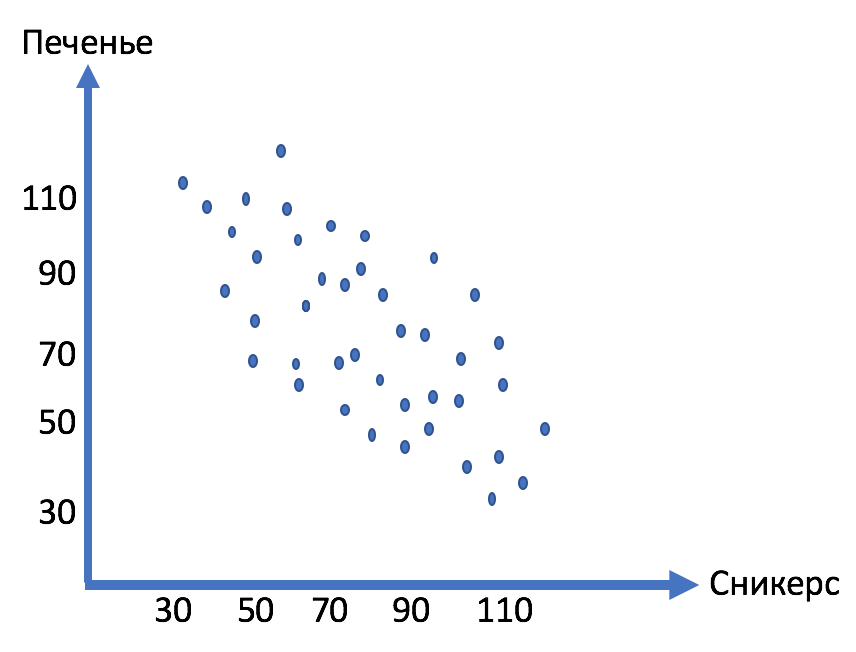
\includegraphics[scale=0.5]{negative_correlation}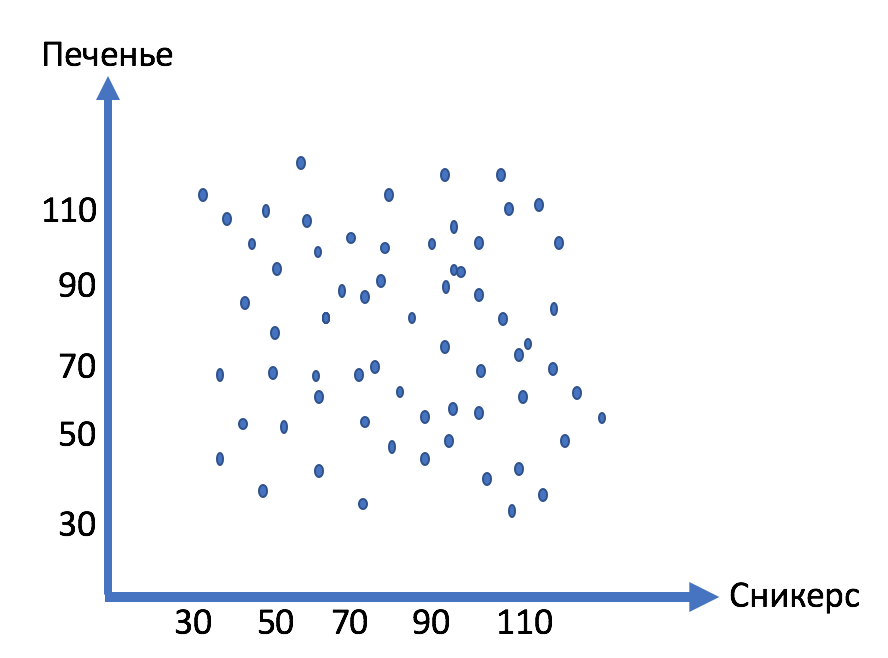
\includegraphics[scale=0.5]{Independent}

\begin{sol}
В первом графике корреляция отрицательная, зависимость существует. Во втором графике $X$ и $Y$ независимые, корреляция равна $0$. 

\end{sol}
\end{problem}

% тур 3 - студия - ковариации и корреляции
\begin{problem}
\item[B2.] Известно, что $\E(X^2)=21,\E(Y) = 2, \Var(X) = 12,\Var(y) = 3, \Corr(X,Y) = \frac{1}{{3}}.$

Найдите $\E(XY)$

\begin{sol}
$8$
\end{sol}
\end{problem}

% тур 3 - студия - ковариации и корреляции
\begin{problem}
\item[B3.] 
Пусть $X$ — доля красных скитлзов в пачке, а $Y$ доля зеленных. Плотность распределения (X,Y) имеет такой вид.

\begin{center} $f_{X,Y}(x,y) = \begin{cases} 6x^2y, & \mbox{при } (x,y) \in [0;1] \times [0;1] \\ 0 , & \mbox{при } (x,y) \not\in [0;1] \times [0;1]\end{cases}$\end{center}

Найдите $\Cov(X,Y)$.

\begin{sol}
$\Cov(X,Y) = \frac{5}{16}$
\end{sol}
\end{problem}

% тур 3 - студия - ковариации и корреляции
\begin{problem}
\item[B4.] Пусть плотность распределения случайной величины $X$ – доли мандаринов среди всех проданных фруктов 31 декабря имеет вид:
\begin{center} $f(x) = \begin{cases} 3x^2, & \mbox{если } x \in [0;1] \\ 0 , & \mbox{иначе }  \end{cases}$  \end{center}
$Y$ — доля проданных мандаринов 1 января, связан с $X$ таким уравнением:

\[Y = \sqrt[]{X}\]

Найдите плотность распределения $Y$.


\begin{sol}
\begin{center} $f(y) = \begin{cases} 6y^5, & \mbox{если } y \in [0;1] \\ 0 , & \mbox{иначе }  \end{cases}$  \end{center}

\end{sol}
\end{problem}
\end{enumerate}


\newpage
\subsection{Тур 3 — студия — Метод первого шага}

\begin{enumerate}
% тур 3 - студия - метод первого шага
\begin{problem}
\item[C1.] Мистер Проппер подкидывает правильную монетку. Если монетка выпадает орлом, Мистер Проппер генерирует случайную величину $\varepsilon=1\;(p=0.5), \varepsilon=-1\;(1-p=0.5)$, если монетка выпадает решкой, Мистер Проппер подкидывает монетку заново. Если монетка на этот раз выпадает орлом, Мистер Проппер генерирует случайную величину $\varepsilon+\nu,\;\; \nu=0\;(p=0.25),\nu=1\;(1-p=0.75)$, иначе подкидывает монетку заново. В общем случае если монетка выпадает орлом на $n$-тое подкидывание, Мистер Проппер генерирует случайную величину $X=\varepsilon+(n-1)\nu$. Найдите $\E(X), \E(X^2)$ методом первого шага, если $\Cov(X,\nu)=1$.

\begin{sol}
$0.75,\; 3.75$
\end{sol}
\end{problem}

% тур 3 - студия - метод первого шага
\begin{problem}
\item[C2.] Мистер Проппер устал от постоянной уборки и решил заглушить свои страдания спиртным и азартными играми. Он приходит в казино с 3 монетами и начинает играть в блэкджек. Партия в блэкджек длится 1 минуту, при этом Мистер Проппер выигрывает партию с вероятностью $p$ и получает 1 монету, либо проигрывает партию с вероятностью $1-p$ и отдаёт 1 монету. Игра в блэкджек заканчивается, когда Мистер Проппер тратит все монеты либо когда на его счету оказывается 4 монеты. Найдите ожидаемое время игры Мистера Проппера  в блэкджек. 

\begin{sol}
$\frac{2p^2-4p+3}{2p^2-2p+1}$
\end{sol}
\end{problem}

% тур 3 - студия - метод первого шага
\begin{problem}
\item[C3.] В разгар веселья Мистера Проппера срочно вызывают ненавистной мелодией 2 нерадивые хозяйки. Он пытается понять, стоит ли ему все отмыть или же отомстить и паркет повредить. Он бросает правильную монетку и если ему выпадает орел, то он портит паркет. Если выпадает решка, то он бросает монетку еще раз. Пусть Х — это сколько раз Мистер Проппер бросает монетку перед тем, как испортить паркет хозяйкам. Найдите $\E(X)$.

\begin{sol}
$2$
\end{sol}
\end{problem}

% тур 3 - студия - метод первого шага
\begin{problem}
\item[C4.] 
После этакого нахальства Мистера Проппера никто не берет на работу. Он одумался и решил извиниться перед хозяйками и отмыть им всю квартиру. Когда он звонит им, они с вероятностью 0.75 принимают извинения, а с вероятностью 0.25 говорят, чтобы он звонил им позже. Если они говорят Мистеру Пропперу, что бы он звонил им позже, он опять бросает правильную монетку и решает звонить им или нет. Он бросает монетку до того момента, пока хозяйки его не простят. Пусть $X$ - количество подбрасываний Мистером Проппером монетки перед тем как звонить хозяйкам. Найдите $\E(X)$.

\begin{sol}
$\frac{8}{3}$
\end{sol}
\end{problem}
\end{enumerate}

\newpage
\subsection{Тур 3 — студия — Оптимальные стратегии}

\begin{enumerate}
% тур 3 - студия - оптимальные стратегии
\begin{problem}
\item[D1.] Ты лежишь на дороге и смертельно ослаб. Спасти тебя может только один вид  целебной лягушки. Целебны у этого вида только самцы. Самцы и самки встречаются равновероятно. Слева в 100 метрах от тебя одна лягушка целебного вида, но не ясно, самец или самка. Справа в 100 метров аж две лягушки целебного вида, но тоже издалека неясно кто. От двух лягушек в твою сторону дует ветер, поэтому ты можешь их слышать.

Самцы и самки квакают по разному, но одинаково часто. Ты слышишь отдельный квак одной из двух лягушек справа и это квак самки.

В какую сторону стоит ползти из последних сил и какова вероятность твоего спасения?

\begin{sol}
D1. Без разницы. Справа условная вероятность спасения при условии отдельного квака равна $1/2$.
\end{sol}
\end{problem}

% тур 3 - студия - оптимальные стратегии
\begin{problem}
\item[D2.] Каждый день племя Виларибо охотится на мамонтов. Охота удачна с вероятностью $0.7$. В племени Виларибо два шамана: шаман Хитрая Игуана и шаман Азартный Бурундук. Каждый из них ни черта не смыслит в охоте на мамонтов, но каждый день вынужден делать прогноз. Если шаман верно угадывает, то ему дарят еду (если мамонт не пойман, то из старых запасов), а если не угадывает, то на племя его громко ругается. Хитрая Игуана предсказывает удачную охоту с вероятностью $\alpha$, а Азартный Бурундук — с вероятностью $\beta$.

Хитрая Игуана максимизирует ожидаемое количество своей еды, какое $\alpha$ ей следует выбрать?

Азартный Бурундук максимизирует дисперсию количества своей еды, какое $\beta$ ему следует выбрать?

\begin{sol}
D2. $\alpha = 1$, $\beta=0.5$
\end{sol}
\end{problem}

% тур 3 - студия - оптимальные стратегии
\begin{problem}
\item[D3.] У племени Вилабаджо тоже есть шаман: Сметливый Туту. От него требуют предсказывать объём мяса, который добудут сегодня на охоте. За прогнозы Сметливый Туту получает 1 кг мяса минус штраф, который равен квадрату ошибки прогноза в тоннах. 

Объём мяса в тоннах, которое каждый день добывает племя — случайная величина с плотностью $f(x)=2-2x$ при $x\in [0;1]$.

Какой прогноз следует высказывать Сметливому Туту, если он хочет получать в среднем побольше мяса от племени?

\begin{sol}
D3. Математическое ожидание минимизирует квадрат ошибки прогноза. Значит берем ожидание, оно равно $\int_0^1 x (2-2x) dx = \frac{1}{3}$.
\end{sol}
\end{problem}


% тур 3 - студия - оптимальные стратегии
\begin{problem}
\item[D4.] Приз в Поле Чудес $X$ равномерно распределен от 0 до 1 миллиона рублей. Лингвист Вася имеет право заранее выбрать порог $b$. Если $X$ окажется больше порога $b$, то лингвист Вася получает $b$. Если $X$ окажется меньше порога $b$, то Вася не получает ничего.

Какой порог следует выбрать Василию?

\begin{sol}
D4. 
\[
\E(b\cdot 1_{X>b})=\int_b^1 b dx \to \max 
\]
Ответ: $b=1/2$

\end{sol}
\end{problem}
\end{enumerate}



\newpage
\subsection{Тур 1 — Мина}


% тур 1 - основная часть - метод первого шага
\begin{enumerate}
\begin{problem}
\item[C4.] Чендлер устроил Джоуи на работу в офис, но Джоуи ничего не знает про статистику. Ему очень скучно, поэтому он любит гулять по офису. Джоуи встаёт со своего рабочего места и с вероятностью $\frac{1}{4}$ идёт на кофепоинт, с вероятностью $\frac{1}{2}$ идёт в туалет, с вероятностью $\frac{1}{4}$ идёт в столовую. Из кофепоинта Джоуи с вероятностями $\frac{1}{3}, \frac{1}{3},\frac{1}{3}$ идёт соответственно на рабочее место, в туалет и в столовую. Из туалета Джоуи с вероятностью $\frac{1}{2}$ идёт на рабочее место,с вероятностью $\frac{1}{4}$ идёт на кофепоинт, с вероятностью $\frac{1}{4}$ идёт в столовую. Наконец, из столовой Джоуи с вероятностью $\frac{2}{3}$ идёт на рабочее место, с вероятностью $\frac{1}{6}$ идёт на кофепоинт, с вероятностью $\frac{1}{6}$ идёт в туалет. Расстояние от рабочего места до столовой Джоуи преодолевает за 3 минуты, до туалета $-$ за 2 минуты, до кофепоинта — за 1 минуту. Расстояние от столовой до кофепоинта Джоуи преодолевает за 3 минуты, до туалета — за 4 минуты. Расстояние от туалета до кофепоинта Джоуи преодолевает за 1 минуту. Найдите ожидаемое время «прогулки» Джоуи до возвращения на рабочее место. 

\begin{sol}
$\frac{509}{76}$
\end{sol}
\end{problem}
\end{enumerate}

\newpage
\subsection{Тур 2 — Мина}

\begin{enumerate}
\begin{problem}
\item[C3.] В кафе Double R Diner начались проблемы: сверхъестественные силы начали вмешиваться в работу таймеров на печах, и теперь вместо \(25\) минут вишневые пироги пекутся \(25 + \varepsilon\) минут, где \(\varepsilon\sim \mathcal{N}(0;1)\). Никто из посетителей пока этого не заметил, однако Норма Дженнингс, владелица кафе, хочет, чтобы ее пироги оставались лучшими в округе, а для этого ей нужно знать, насколько в среднем ошибаются таймеры на печах и как оценивать другие характеристики. Помогите Норме: найдите $f_{|\varepsilon|}(x)$ и $\E(|\varepsilon|)$.

\begin{sol}
$f_{|\varepsilon|}(x) = 2f_{\varepsilon}(x) \cdot \mathcal{I} \{\varepsilon \geq 0\}$, $\sqrt{\frac{2}{\pi}}$
\end{sol}
\end{problem}
\end{enumerate}

\newpage
\subsection{Тур 3 — Мина}

\begin{enumerate}
\begin{problem}
\item[B4.] Кардиналу Войелло очень не нравится, что Папа Пий XIII не делает публичных выступлений. На досуге он обдумывал хитрый план: подговорить Софию и продать интервью с Папой первому человеку, который предложит $130000$ евро. В его воображаемой модели предложения – независимые случайный величины, распределённые экспоненциально со средним $100000$.

Найдите ожидаемое число предложений.

\begin{sol}
$e^{1.3} \approx 4.5$
\end{sol}
\end{problem}
\end{enumerate}


\end{document}
